\documentclass[conference]{IEEEtran}
\IEEEoverridecommandlockouts
\usepackage[T1]{fontenc}
\usepackage{cite}
\usepackage{amsmath,amssymb,amsfonts}
\usepackage{algorithmic}
\usepackage{algorithm}
\usepackage{graphicx}
\usepackage{booktabs}
\usepackage{multirow}
\usepackage{xcolor}
\usepackage[hidelinks]{hyperref}
\graphicspath{{figures/}}
\setlength{\emergencystretch}{2em}
% primitive \input so table bodies (generated by make_tables.py) work inside tabular
\makeatletter\newcommand{\tabinput}[1]{\@@input #1 }\makeatother
\newcommand{\Tsel}{T_{\mathrm{sel}}}
\newcommand{\Tsub}{T_{\mathrm{sub}}}
\newcommand{\Tfull}{T_{\mathrm{full}}}

\begin{document}

\title{Gradient-Matching Coreset Selection for Data-Efficient Training: A Reproduction and Runtime Break-Even Analysis of CRAIG}

\author{\IEEEauthorblockN{Harsh Joshi}\and\IEEEauthorblockN{Mayank Srivastava}\and\IEEEauthorblockN{Zayed Alam}\and\IEEEauthorblockN{Himesh}}

\maketitle

\begin{abstract}
CRAIG selects a weighted subset (coreset) of the training data whose weighted gradient sum approximates the full-data gradient, by greedily maximizing a submodular facility-location objective over pairwise per-sample gradient distances~\cite{mirzasoleiman2020craig}. We re-implement CRAIG from scratch in PyTorch~\cite{paszke2019pytorch} and evaluate it on a CPU-only machine. We account for the full wall-clock cost: per-sample gradients, pairwise similarities, greedy selection, weight assignment, and training on the subset. Unlike the original deep-network protocol, our selection is performed once, at the initial weights, with no per-epoch re-selection. On MNIST with logistic regression (5 seeds), weighted CRAIG has a higher mean accuracy than uniform random subsets at every subset ratio from 5\% to 50\%, e.g., $90.19\pm0.15\%$ vs.\ $89.68\pm0.18\%$ at 5\% (full data: $92.22\pm0.12\%$). Without its weights, CRAIG is worse than random. However, selection takes 29.41--38.20\,s against 6.58\,s for full training, so the end-to-end speedup is only 0.16--0.22$\times$: CRAIG is \emph{slower} than full training. The lazy-greedy step accounts for 77--81\% of the selection time. A dataset-size scaling study places the break-even point between $N{=}5{,}000$ and $N{=}10{,}000$ samples in our setup. On a reduced CIFAR-10 setting (10k training images, 3 seeds), CRAIG has a much lower gradient approximation error than random sampling (0.207 vs.\ 0.802 at 10\%). Yet it beats random in accuracy only at the 10\% ratio. On synthetic time series, accuracy results are too unstable to support a conclusion. We report these negative results explicitly and discuss when gradient-matching coresets can pay off.
\end{abstract}

\begin{IEEEkeywords}
coresets, data subset selection, submodular optimization, facility location, data-efficient training, reproducibility
\end{IEEEkeywords}

%======================================================================
\section{Introduction}
%======================================================================
Training cost grows with the size of the training set. One way to reduce it is to train on a small, carefully chosen subset. Mirzasoleiman, Bilmes, and Leskovec proposed CRAIG (\emph{Coresets for Accelerating Incremental Gradient descent})~\cite{mirzasoleiman2020craig}. CRAIG selects a subset $S$ and per-element weights such that the weighted subset gradient approximates the full gradient. The selection problem is cast as maximizing a monotone submodular facility-location function. Greedy maximization of such a function enjoys a $(1-1/e)$ approximation guarantee~\cite{nemhauser1978analysis}.

A coreset method helps in practice only if the time spent \emph{selecting} the subset, plus the time spent training on it, is less than the time for training on the full data. This report is a reproduction of CRAIG. It is designed around that end-to-end accounting and run on commodity CPU hardware. Our contributions are:
\begin{itemize}
\item A from-scratch, tested implementation of the CRAIG pipeline. It computes exact per-sample gradients with \texttt{torch.func} (\texttt{vmap} over \texttt{grad}), builds blockwise gradient-distance matrices, runs naive and lazy~\cite{minoux1978accelerated} greedy facility location, and assigns Voronoi weights $w_j=|C_j|$.
\item A benchmark on MNIST~\cite{lecun1998gradient} (logistic regression, full 60k training set, 5 seeds), a reduced-scale CIFAR-10~\cite{krizhevsky2009learning} experiment, and synthetic time-series data. It compares weighted CRAIG, unweighted CRAIG, uniform random subsets, and full-data training.
\item A per-stage runtime breakdown and a break-even analysis, including scaling with dataset size and sequence length.
\end{itemize}
Our main finding is mixed. The \emph{statistical} part of CRAIG reproduces on MNIST: weighted coresets reach higher mean accuracy than random subsets of equal size, and the weights are essential. The \emph{computational} claim does not hold in our setting: with a pure-Python lazy greedy on CPU, selection is 4.47--5.80$\times$ more expensive than full training. All experiments were run on a CPU-only machine. Several experiments are at reduced scale, as detailed in Section~\ref{sec:setup}.

%======================================================================
\section{Related Work}
%======================================================================
\textbf{Submodular maximization.} Nemhauser, Wolsey, and Fisher~\cite{nemhauser1978analysis} showed that the greedy algorithm achieves a $(1-1/e)$ approximation for maximizing a monotone submodular set function under a cardinality constraint. Minoux~\cite{minoux1978accelerated} introduced the \emph{lazy} (accelerated) greedy algorithm. It exploits the diminishing-returns property: marginal gains computed in earlier iterations remain valid upper bounds. As a result, most candidates need not be re-evaluated, and the selected set is identical to the naive greedy one, up to ties.

\textbf{Coresets for training.} CRAIG~\cite{mirzasoleiman2020craig} connects these results to incremental gradient methods. It bounds the error between the full gradient and a weighted subset gradient by a facility-location objective over per-sample gradient differences. It then selects the subset greedily and trains on it with weighted incremental gradient updates. For convex problems, the original work bounds gradient differences by feature-space distances, which do not depend on the parameters. For deep networks, it uses an approximation based on last-layer gradients and re-selects the subset during training. Our work is a reproduction of this method only. We do not compare against other subset-selection families, such as importance sampling or active learning, and we make no claims about them.

\textbf{Tooling.} Our implementation relies on PyTorch~\cite{paszke2019pytorch}, including its functional transforms (\texttt{torch.func}) for vectorized per-sample gradients.

%======================================================================
\section{Background: CRAIG}
\label{sec:background}
%======================================================================
Let $V=\{(x_i,y_i)\}_{i=1}^N$ be the training set and $\ell_i(\theta)$ the loss of sample $i$ under parameters $\theta\in\mathbb{R}^D$. Let $g_i(\theta)=\nabla_\theta\ell_i(\theta)$ be its per-sample gradient. The full gradient of the empirical risk is $G_V(\theta)=\frac{1}{N}\sum_{i\in V}g_i(\theta)$. A weighted coreset $S\subseteq V$, $|S|=k\ll N$, with weights $w_j\ge 0$, gives the approximation $G_S(\theta)=\frac{1}{N}\sum_{j\in S}w_j g_j(\theta)$.

\textbf{Gradient matching.} Partition $V$ into clusters $\{C_j\}_{j\in S}$, one per representative, and set $w_j=|C_j|$, so that $\sum_j w_j=N$. By the triangle inequality,
\begin{equation}
\|G_V-G_S\| \le \frac{1}{N}\sum_{j\in S}\sum_{i\in C_j}\|g_i-g_j\|.
\label{eq:bound}
\end{equation}
The bound is minimized by assigning each $i$ to its closest representative. Selecting $S$ then becomes a $k$-medoids problem, $\min_{|S|\le k}\sum_{i\in V}\min_{j\in S} d(i,j)$, with $d(i,j)=\|g_i-g_j\|$.

\textbf{Facility location.} With $M\ge\max_{i,j}d(i,j)$ and similarity $s(i,j)=M-d(i,j)\ge 0$, minimizing~\eqref{eq:bound} is equivalent to maximizing
\begin{equation}
F(S)=\sum_{i\in V}\max_{j\in S}s(i,j).
\label{eq:fl}
\end{equation}
$F$ is monotone and submodular. Greedy selection, which repeatedly adds $j^\star=\arg\max_c F(S\cup\{c\})-F(S)$, therefore achieves at least $(1-1/e)$ of the optimal value~\cite{nemhauser1978analysis}. After selection, every $i$ is assigned to $\arg\max_{j\in S}s(i,j)$ (a Voronoi assignment), and $w_j=|C_j|$.

\textbf{Evaluation quantities.} We measure the gradient approximation quality at the parameters used for selection by the relative error $\|\sum_i g_i-\sum_{j\in S}w_jg_j\|/\|\sum_i g_i\|$ and by the cosine similarity between the two sums. For random or unweighted subsets we use the uniform weights $w_j=N/k$. The run time of CRAIG is $T_{\mathrm{CRAIG}}=\Tsel+\Tsub$, where $\Tsel$ includes gradients, similarity, greedy selection, and weight assignment. We report the training-only speedup $\Tfull/\Tsub$ and the end-to-end speedup $\Tfull/(\Tsel+\Tsub)$. A true computational win requires $\Tsel<\Tfull-\Tsub$.

%======================================================================
\section{Method and Implementation}
\label{sec:method}
%======================================================================
The implementation lives in the \texttt{craig/} package of the project repository. A unit-test suite covers gradients, similarity, facility location, the selector, and training; all 23 tests pass.

\textbf{Per-sample gradients.} The module \texttt{craig/\allowbreak gradients.py} computes the $N\times D$ gradient matrix. It applies \texttt{torch.func.vmap} over \texttt{torch.func.grad} of a single-sample loss evaluated through \texttt{functional\_call}, processing chunks of 64--128 samples to bound memory. If vectorization fails, the code falls back to one backward pass per sample; it never reuses a batch gradient for individual samples. Gradients are computed with the model in evaluation mode, so BatchNorm layers use their running statistics.

\textbf{Representations.} The module \texttt{craig/\allowbreak representations.py} supports three representations: the full parameter gradient; the gradient of the final linear (classifier) layer only; and an optional Johnson--Lindenstrauss random projection (Gaussian or Rademacher). The projection was not used in the reported experiments. We use the full gradient for logistic regression ($D=7{,}850$) and for the 1D time-series CNN ($D=23{,}492$). For the CIFAR-10 CNN we use last-layer gradients ($D=1{,}290$).

\textbf{Similarity.} The module \texttt{craig/\allowbreak similarity.py} computes Euclidean (or cosine) distances blockwise, using $\|x\|^2+\|y\|^2-2x^\top y$ on row blocks of 1024. A 4\,GiB guard limits the size of the dense matrix. Similarities are $s=\max(D)-D$, where the maximum is taken within the matrix being built.

\textbf{Greedy facility location.} The module \texttt{craig/\allowbreak facility\_\allowbreak location.py} provides a naive vectorized greedy algorithm and a lazy greedy algorithm (Alg.~\ref{alg:lazy})~\cite{minoux1978accelerated}. The lazy variant keeps a max-heap of stale marginal gains. It recomputes the gain of the top candidate and accepts it if it is still at least the next-best upper bound. The lazy variant was used in all experiments.

\begin{algorithm}[t]
\caption{Lazy greedy facility location (per class)}
\label{alg:lazy}
\begin{algorithmic}[1]
\REQUIRE similarity matrix $s\in\mathbb{R}_{\ge0}^{n\times n}$, budget $k$
\STATE $c\leftarrow \mathbf{0}_n$ \COMMENT{current coverage $\max_{j\in S}s(i,j)$}
\STATE push $(\sum_i s(i,j),\,j)$ for all $j$ into max-heap $H$; $S\leftarrow\emptyset$
\WHILE{$|S|<k$}
  \STATE pop $(\cdot,j)$ from $H$; $\delta\leftarrow\sum_i\max(0,s(i,j)-c_i)$
  \IF{$H=\emptyset$ \textbf{or} $\delta\ge$ top bound of $H$}
    \STATE $S\leftarrow S\cup\{j\}$; $c\leftarrow\max(c,s(\cdot,j))$
  \ELSE
    \STATE push $(\delta,j)$ back into $H$
  \ENDIF
\ENDWHILE
\STATE $w_j\leftarrow|\{i:\arg\max_{j'\in S}s(i,j')=j\}|$ for $j\in S$
\RETURN $S$, $w$
\end{algorithmic}
\end{algorithm}

\textbf{CraigSelector.} \texttt{craig/\allowbreak selector.py} runs the pipeline gradients $\rightarrow$ similarity $\rightarrow$ greedy $\rightarrow$ weights. Selection is done \emph{per class}: each class $c$ with $n_c$ samples receives a budget of $\mathrm{round}(k\,n_c/N)$. This keeps the dense matrices at size $n_c\times n_c$. Because of the rounding, the realized CRAIG subset size can differ from $k$ by a few samples; for example, it is 5,999 instead of 6,000 at 10\% on MNIST. Every stage is timed with \texttt{time.perf\_counter}, with device synchronization if a GPU is used.

\textbf{Weighted training.} When weights are used, the minibatch loss is $\sum_{i\in B}w_i\ell_i/\sum_{i\in B}w_i$. This is a per-minibatch normalized weighted loss. It is a simplification of the weighted incremental-gradient step sizes described in~\cite{mirzasoleiman2020craig}. CRAIG-unweighted trains on the same subset with the standard mean loss.

%======================================================================
\section{Experimental Setup}
\label{sec:setup}
%======================================================================
\textbf{Hardware and software.} All runs used a single Linux machine with 8 CPU cores (Intel Xeon) and a CPU-only PyTorch build (2.15.0+cpu). No GPU or Apple-MPS runs were performed. Device-selection code paths for those backends exist but are untested. All times are wall-clock seconds. The machine was not isolated, so the timings contain noise: for example, the standard deviation of full CIFAR-10 training time across seeds is 3.90\,s on a mean of 13.17\,s.

\textbf{Methods.} We compare four methods. FULL trains on all $N$ samples. RANDOM trains on a uniform random subset of size $k$, with unweighted loss. CRAIG trains on the CRAIG subset with weights $w_j=|C_j|$. CRAIG-unweighted trains on the same subset as CRAIG but without weights. All methods share the optimizer, learning rate, batch size, number of epochs, and model initialization for a given seed. $\Tsel$ is recomputed for every (seed, ratio) pair; nothing is cached. Test-set evaluation is excluded from the training time.

\textbf{Selection protocol.} CRAIG selects \emph{once}, using gradients at the seed's initial weights. The same initialization is then trained on the subset. This is a deliberate simplification. For deep networks, the original method re-selects the subset during training~\cite{mirzasoleiman2020craig}. For convex models, it uses a parameter-independent feature-space bound instead of exact gradients at a particular $\theta$.

\textbf{MNIST}~\cite{lecun1998gradient}. We train multinomial logistic regression ($784\rightarrow10$) on the full 60k training set and evaluate on the 10k test set. Inputs are normalized. We use SGD (lr 0.01, momentum 0.9, weight decay $10^{-4}$), batch size 128, and 20 epochs. Seeds are $\{42,123,456,789,1000\}$ and subset ratios are $\{5,10,20,30,50\}\%$. CRAIG uses full gradients and Euclidean distance.

\textbf{CIFAR-10}~\cite{krizhevsky2009learning} \emph{(reduced scale).} We use only the first 10,000 training images and the full 10k test set, with per-channel normalization and no augmentation. The model is a small CNN with two $3\times3$ conv layers (32 and 64 channels, each followed by max-pooling) and fully connected layers $4096\rightarrow128\rightarrow10$, for 545,098 parameters in total. We use SGD (lr 0.01, momentum 0.9, weight decay $5\times10^{-4}$), batch size 128, and 10 epochs. Seeds are $\{42,123,456\}$ and ratios are $\{10,20,30,50\}\%$. CRAIG uses last-layer gradients. This setting is far from the original paper's CIFAR-10 setup, and FULL reaches only 59.02\%.

\textbf{Synthetic time series.} No real time-series dataset (e.g., from the UCR archive) was available, so we use a synthetic generator. A sample of class $c\in\{0,1,2,3\}$ is $\sin(2\pi f_c t+\phi)+\varepsilon$, with $f_c=2(c+1)$, a random phase $\phi$, and Gaussian noise $\varepsilon\sim\mathcal{N}(0,\sigma^2)$. Each sequence has $L=100$ points, the training set has $N=4{,}000$ sequences, and the test set has 1,000. The model is a 1D CNN with three conv+BatchNorm layers, global average pooling, and a linear head. We train with Adam (lr $10^{-3}$, weight decay $10^{-4}$), batch size 64, for 10 epochs, with 3 seeds and the same five ratios as MNIST. We run an \emph{easy} setting ($\sigma{=}0.2$) and a \emph{hard} setting ($\sigma{=}2.0$).

\textbf{Scaling studies} (2 seeds $\{42,123\}$, ratio 10\%, 10 epochs, FULL/RANDOM/CRAIG only). In the \emph{dataset-size} study, we train MNIST logistic regression on the first $N\in\{1{,}000,\ldots,20{,}000\}$ training images, with the same optimizer as above. In the \emph{sequence-length} study, we use the synthetic time series ($\sigma{=}0.2$) with $N{=}2{,}000$ and $L\in\{50,100,200,500,1000\}$.

All numbers below are computed directly from the experiment CSV files (\texttt{results/raw}, \texttt{results/processed}) by a script, \texttt{paper/make\_tables.py}, that emits the table bodies. Means $\pm$ sample standard deviations are taken over seeds. Speedups are ratios of mean times.

%======================================================================
\section{Results}
\label{sec:results}
%======================================================================
\subsection{MNIST: accuracy}

\begin{table}[t]
\centering
\caption{MNIST logistic regression: test accuracy (\%), mean $\pm$ std over 5 seeds. $k$ is the RANDOM subset size; CRAIG's per-class rounding gives $k{\pm}1$.}
\label{tab:mnist_acc}
\setlength{\tabcolsep}{4pt}
\begin{tabular}{@{}lrccc@{}}
\toprule
Ratio & $k$ & CRAIG & CRAIG-unw. & RANDOM \\
\midrule
\tabinput{tables/mnist_acc.tex}
\bottomrule
\end{tabular}
\end{table}

\begin{figure}[t]
\centering
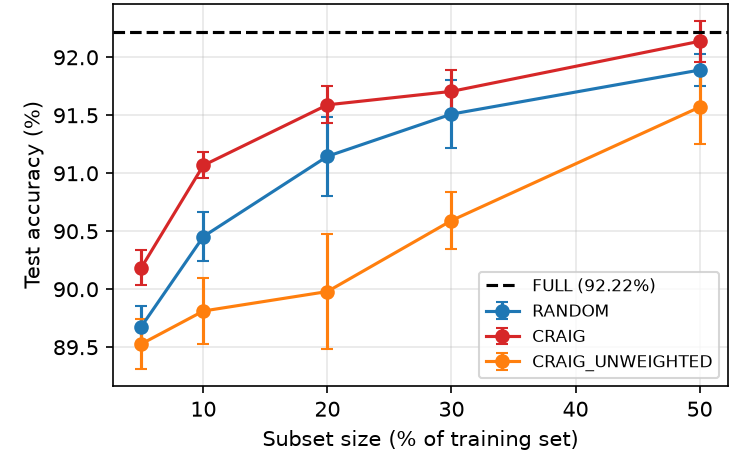
\includegraphics[width=\columnwidth]{mnist_acc_vs_ratio.png}
\caption{MNIST: test accuracy vs.\ subset size (mean $\pm$ std, 5 seeds). The dashed line is FULL ($92.22\%$).}
\label{fig:mnist_acc}
\end{figure}

Table~\ref{tab:mnist_acc} and Fig.~\ref{fig:mnist_acc} show that weighted CRAIG has the highest mean accuracy among the subset methods at every ratio. At 50\% it comes within 0.08 points of FULL ($92.14\pm0.18\%$ vs.\ $92.22\pm0.12\%$). Because all methods share the seed, we also report paired per-seed differences (Table~\ref{tab:paired}). CRAIG beats RANDOM in 5/5 seeds at 5--20\% (by $+0.44$ to $+0.61$ points on average). At 30\% and 50\% it wins in only 4/5 seeds, and the mean gaps ($+0.20$, $+0.25$) are comparable to the seed-to-seed spread. The weights matter: CRAIG-unweighted trains on exactly the same points but is \emph{below} RANDOM at every ratio. Weighted CRAIG beats it in 5/5 seeds at every ratio, by $+0.57$ to $+1.61$ points.

\begin{table}[t]
\centering
\caption{Paired per-seed accuracy difference of weighted CRAIG vs.\ the baseline (percentage points, mean $\pm$ std; in parentheses, the number of seeds where CRAIG is higher). $^\dagger$Reduced scale.}
\label{tab:paired}
\footnotesize
\setlength{\tabcolsep}{3pt}
\begin{tabular}{@{}llcc@{}}
\toprule
Data & Ratio & CRAIG$-$RANDOM & CRAIG$-$CRAIG-unw. \\
\midrule
\tabinput{tables/paired.tex}
\bottomrule
\end{tabular}
\end{table}

\subsection{MNIST: gradient approximation error}

\begin{table}[t]
\centering
\caption{MNIST: relative gradient error at the initial weights (mean $\pm$ std, 5 seeds) and mean cosine similarity between $\sum_i g_i$ and the subset estimate.}
\label{tab:mnist_gerr}
\footnotesize
\setlength{\tabcolsep}{2pt}
\begin{tabular}{@{}lccccc@{}}
\toprule
 & \multicolumn{3}{c}{Relative error} & \multicolumn{2}{c}{Cosine} \\
\cmidrule(lr){2-4}\cmidrule(lr){5-6}
Ratio & CRAIG & CRAIG-unw. & RANDOM & CRAIG & RANDOM \\
\midrule
\tabinput{tables/mnist_gerr.tex}
\bottomrule
\end{tabular}
\end{table}

On MNIST, the gradient error of weighted CRAIG is only marginally below that of RANDOM (Table~\ref{tab:mnist_gerr}): 0.118 vs.\ 0.128 at 5\% and 0.027 vs.\ 0.030 at 50\%. Its seed-to-seed spread is several times smaller. The unweighted CRAIG estimate (same points, uniform weights $N/k$) behaves very differently. Its error \emph{grows} from 0.110 at 5\% to 0.203 at 30\%. This shows that the medoids alone are a biased sample of the gradient distribution, and that the Voronoi weights $w_j=|C_j|$ correct the bias.

\begin{figure*}[t]
\centering
\begin{minipage}[t]{0.49\textwidth}\centering
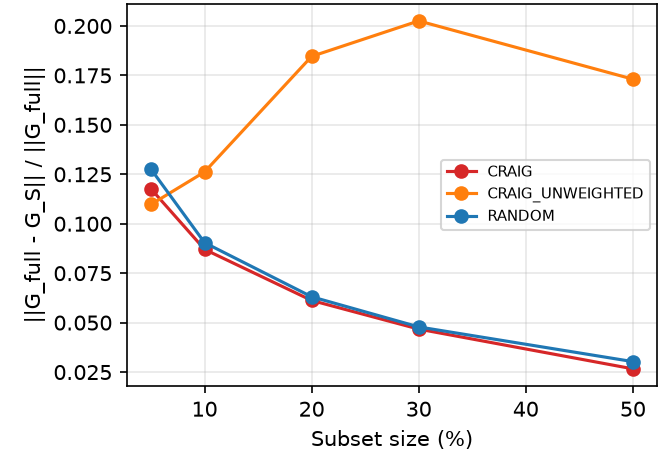
\includegraphics[width=\linewidth]{mnist_grad_err_rel.png}\\
\small (a) MNIST (5 seeds)
\end{minipage}\hfill
\begin{minipage}[t]{0.49\textwidth}\centering
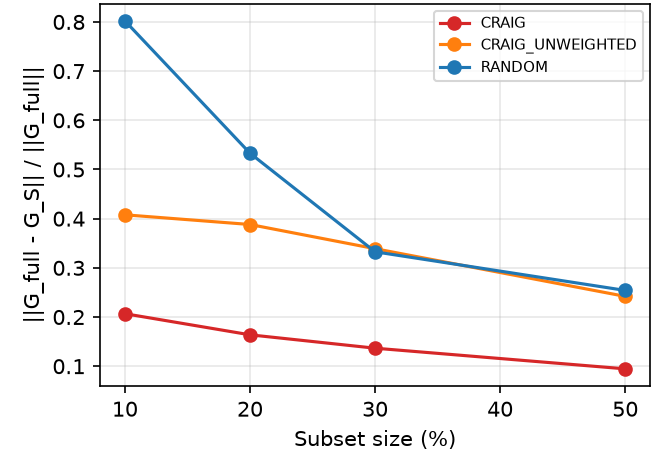
\includegraphics[width=\linewidth]{cifar10_grad_err_rel.png}\\
\small (b) CIFAR-10, reduced scale (3 seeds, last-layer gradients)
\end{minipage}
\caption{Relative gradient approximation error $\|G_V-G_S\|/\|G_V\|$ at the initial weights vs.\ subset size. Weighted CRAIG has a lower error than RANDOM at every ratio. The gap is small on MNIST and large on CIFAR-10. On MNIST at 5\%, the unweighted estimate is slightly lower (0.110 vs.\ 0.118).}
\label{fig:gerr}
\end{figure*}

\subsection{MNIST: time breakdown and break-even}

\begin{table*}[t]
\centering
\caption{MNIST: mean CRAIG time per stage (s, 5 seeds). ``Weights'' $=\Tsel-(\text{gradients}+\text{similarity}+\text{greedy})$ is the Voronoi weight-assignment time. Speedups are relative to FULL training ($\Tfull=6.58$\,s).}
\label{tab:mnist_time}
\setlength{\tabcolsep}{4.5pt}
\begin{tabular}{@{}lccccccccc@{}}
\toprule
Ratio & Gradients & Similarity & Lazy greedy & Weights & $\Tsel$ (mean$\pm$std) & $\Tsub$ & $\Tsel+\Tsub$ & Train-only speedup & End-to-end speedup \\
\midrule
\tabinput{tables/mnist_time.tex}
\bottomrule
\end{tabular}
\end{table*}

Table~\ref{tab:mnist_time} and Figs.~\ref{fig:mnist_time} and~\ref{fig:mnist_speedup} give the main negative result. Training on the coreset is 1.58--14.29$\times$ faster than full training. Selection, however, takes 29.41--38.20\,s, which is 4.47--5.80$\times$ the 6.58\,s full-training time. The end-to-end speedup is therefore 0.16--0.22$\times$, and CRAIG does \emph{not} break even at any ratio on MNIST. RANDOM, whose selection costs below 2\,ms, has end-to-end speedups of 1.98--19.62$\times$.

The lazy greedy step dominates selection: it takes 22.71--29.33\,s, or 77--81\% of $\Tsel$. Similarity computation takes 13--18\%, and the vectorized per-sample gradients only about 1\,s (2.7--3.7\%). Selection time also varies substantially across seeds (std 3.88--7.17\,s).

\begin{figure}[t]
\centering
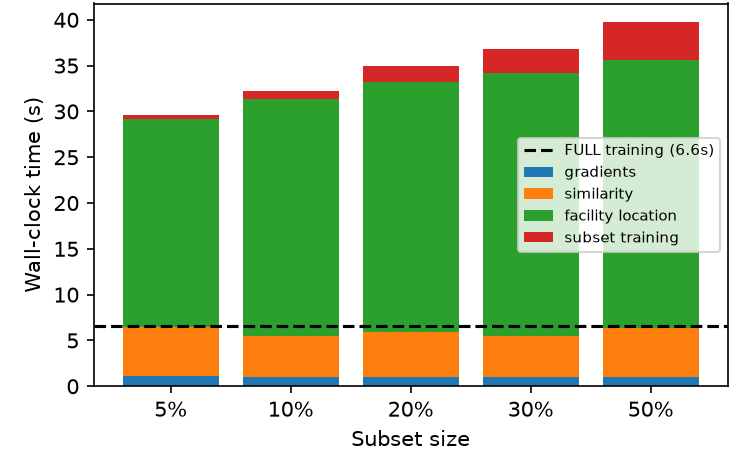
\includegraphics[width=\columnwidth]{mnist_time_breakdown.png}
\caption{MNIST: mean CRAIG wall-clock time by stage (5 seeds). The dashed line is FULL training (6.6\,s). The weight-assignment component of Table~\ref{tab:mnist_time} is not drawn.}
\label{fig:mnist_time}
\end{figure}

\begin{figure}[t]
\centering
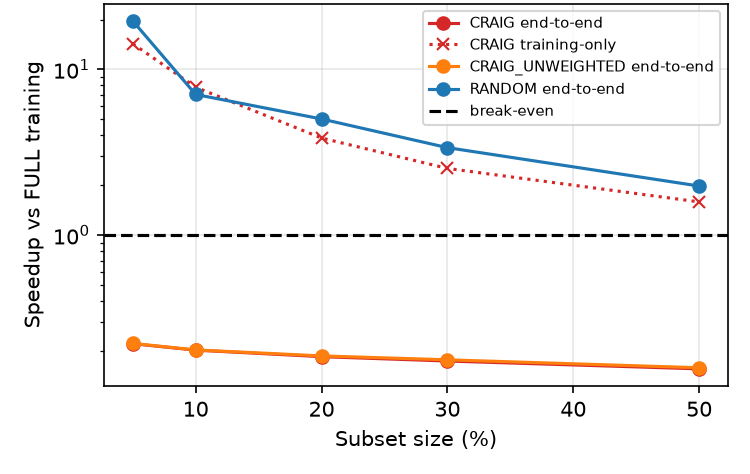
\includegraphics[width=\columnwidth]{mnist_speedup.png}
\caption{MNIST: speedup relative to FULL training (log scale). CRAIG's training-only speedup is above 1, but its end-to-end speedup (selection included) is 0.16--0.22$\times$, below the break-even line. The curves for weighted and unweighted CRAIG overlap.}
\label{fig:mnist_speedup}
\end{figure}

\subsection{CIFAR-10 (reduced scale)}

\begin{figure*}[t]
\centering
\begin{minipage}[t]{0.49\textwidth}\centering
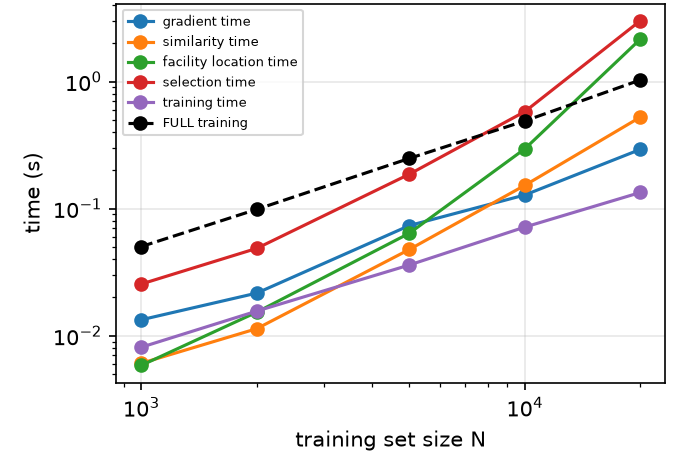
\includegraphics[width=\linewidth]{scaling_size_cost.png}\\
\small (a) MNIST logistic regression, training-set size $N$
\end{minipage}\hfill
\begin{minipage}[t]{0.49\textwidth}\centering
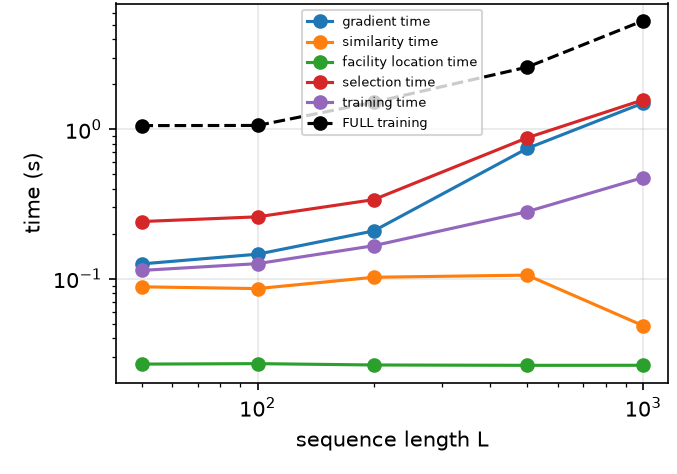
\includegraphics[width=\linewidth]{scaling_seq_cost.png}\\
\small (b) Synthetic time series ($N{=}2{,}000$), sequence length $L$
\end{minipage}
\caption{Scaling of CRAIG's cost (ratio 10\%, 10 epochs, mean over 2 seeds, log--log axes). The curves show the CRAIG stage times, CRAIG subset training (``training time''), and FULL training (dashed). In (a), selection overtakes FULL training between $N{=}5{,}000$ and $N{=}10{,}000$. In (b), only the gradient time grows with $L$. Accuracies are given in Table~\ref{tab:scaling}.}
\label{fig:scaling}
\end{figure*}

\begin{table*}[t]
\centering
\caption{Scaling studies (ratio 10\%, 10 epochs, 2 seeds). Top: MNIST logistic regression with training-set size $N$ (mean accuracies). Bottom: synthetic time series ($\sigma{=}0.2$, $N{=}2000$) with sequence length $L$ (accuracies as mean $\pm$ std). Times are mean seconds; accuracies are in \%.}
\label{tab:scaling}
\begin{tabular}{@{}rccccccccc@{}}
\toprule
$N$ & $T_{\mathrm{grad}}$ & $T_{\mathrm{sim}}$ & $T_{\mathrm{FL}}$ & $\Tsel$ & $\Tfull$ & CRAIG end-to-end speedup & CRAIG acc. & RANDOM acc. & FULL acc. \\
\midrule
\tabinput{tables/scaling_size.tex}
\midrule
$L$ & $T_{\mathrm{grad}}$ & $T_{\mathrm{sim}}$ & $T_{\mathrm{FL}}$ & $\Tsel$ & $\Tfull$ & CRAIG end-to-end speedup & CRAIG acc. & RANDOM acc. & FULL acc. \\
\midrule
\tabinput{tables/scaling_seq.tex}
\bottomrule
\end{tabular}
\end{table*}


\begin{table}[t]
\centering
\caption{CIFAR-10, reduced scale (10k training images, 10 epochs): test accuracy (\%), mean $\pm$ std over 3 seeds.}
\label{tab:cifar_acc}
\setlength{\tabcolsep}{4pt}
\begin{tabular}{@{}lrccc@{}}
\toprule
Ratio & $k$ & CRAIG & CRAIG-unw. & RANDOM \\
\midrule
\tabinput{tables/cifar_acc.tex}
\bottomrule
\end{tabular}
\end{table}

\begin{table}[t]
\centering
\caption{CIFAR-10 (reduced): relative gradient error (mean $\pm$ std), CRAIG gradient time, $\Tsel$, $\Tsub$ (s), and CRAIG end-to-end speedup.}
\label{tab:cifar_time}
\setlength{\tabcolsep}{2.2pt}
\begin{tabular}{@{}lcccccc@{}}
\toprule
 & \multicolumn{2}{c}{Rel.\ grad.\ error} & & & & \\
\cmidrule(lr){2-3}
Ratio & CRAIG & RANDOM & $T_{\mathrm{grad}}$ & $\Tsel$ & $\Tsub$ & E2E \\
\midrule
\tabinput{tables/cifar_gerr_time.tex}
\bottomrule
\end{tabular}
\end{table}

\begin{figure}[t]
\centering
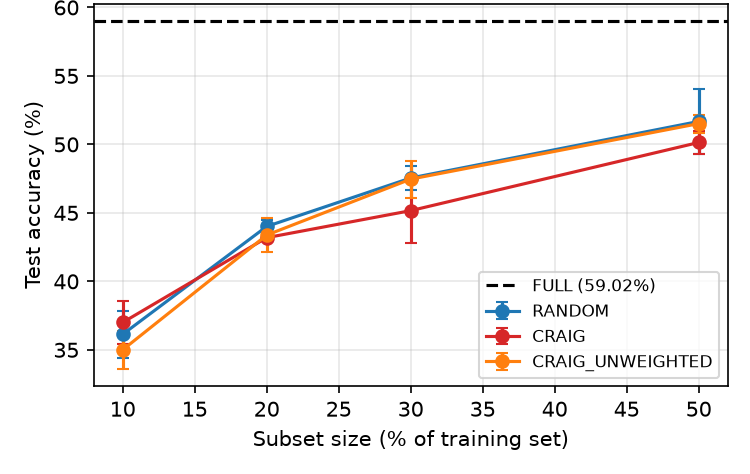
\includegraphics[width=\columnwidth]{cifar10_acc_vs_ratio.png}
\caption{CIFAR-10 (reduced scale): test accuracy vs.\ subset size (mean $\pm$ std, 3 seeds). The dashed line is FULL (59.02\%).}
\label{fig:cifar_acc}
\end{figure}

On reduced CIFAR-10 (Tables~\ref{tab:cifar_acc} and~\ref{tab:cifar_time}, Figs.~\ref{fig:gerr}b and~\ref{fig:cifar_acc}), last-layer CRAIG approximates the last-layer gradient far better than random sampling: the relative error is 0.207 vs.\ 0.802 at 10\% and 0.095 vs.\ 0.254 at 50\%. This does \emph{not} translate into accuracy. CRAIG beats RANDOM only at 10\% ($37.00\pm1.58\%$ vs.\ $36.13\pm1.71\%$; 3/3 seeds). It is lower at 20\%, 30\%, and 50\%, by 0.82 to 2.38 points on average (Table~\ref{tab:paired}). All subset accuracies remain 7.3--24.0 points below FULL ($59.02\pm0.17\%$). Selection is cheap here, about 1\,s, because $D=1{,}290$ and each class has only about 1,000 samples. CRAIG therefore breaks even at every ratio (end-to-end speedup 1.75--5.07$\times$). RANDOM is still faster at matching or higher accuracy. We attribute the accuracy result mainly to the one-shot selection at a random initialization. At that point, last-layer gradients describe an untrained network, so a subset that matches them need not stay representative as the features change.

\subsection{Synthetic time series}

In the easy setting ($\sigma{=}0.2$), every method reaches 100\% test accuracy at every ratio and seed. The task therefore cannot separate the methods. Table~\ref{tab:ts} and Fig.~\ref{fig:ts} report the hard setting ($\sigma{=}2.0$). Here the results are unstable. FULL reaches only $52.87\pm5.90\%$, below several subset configurations. At 30\% and 50\%, the standard deviations reach 11.9--16.5 points. Weighted CRAIG has a higher mean than RANDOM only at 20\%. No reliable accuracy conclusion can be drawn; the training setup needs tuning, and BatchNorm instability between training and evaluation is one plausible cause. The gradient-matching objective itself still behaves as expected. CRAIG's relative gradient error is roughly an order of magnitude below RANDOM's (e.g., 0.070 vs.\ 0.662 at 10\%). Selection costs about 0.7\,s against 2.52\,s for full training, so CRAIG breaks even at every ratio (1.38--2.92$\times$).

\begin{table}[t]
\centering
\caption{Synthetic time series, hard setting ($\sigma{=}2.0$, $N{=}4000$, $L{=}100$, 3 seeds). Top: test accuracy (\%). Bottom: relative gradient error, $\Tsel$, $\Tsub$ (s), and CRAIG end-to-end speedup.}
\label{tab:ts}
\setlength{\tabcolsep}{3pt}
\begin{tabular}{@{}lrccc@{}}
\toprule
Ratio & $k$ & CRAIG & CRAIG-unw. & RANDOM \\
\midrule
\tabinput{tables/ts_hard_acc.tex}
\bottomrule
\end{tabular}\\[4pt]
\begin{tabular}{@{}lccccc@{}}
\toprule
 & \multicolumn{2}{c}{Rel.\ grad.\ error} & & & \\
\cmidrule(lr){2-3}
Ratio & CRAIG & RANDOM & $\Tsel$ & $\Tsub$ & E2E \\
\midrule
\tabinput{tables/ts_hard_gerr_time.tex}
\bottomrule
\end{tabular}
\end{table}

\begin{figure}[t]
\centering
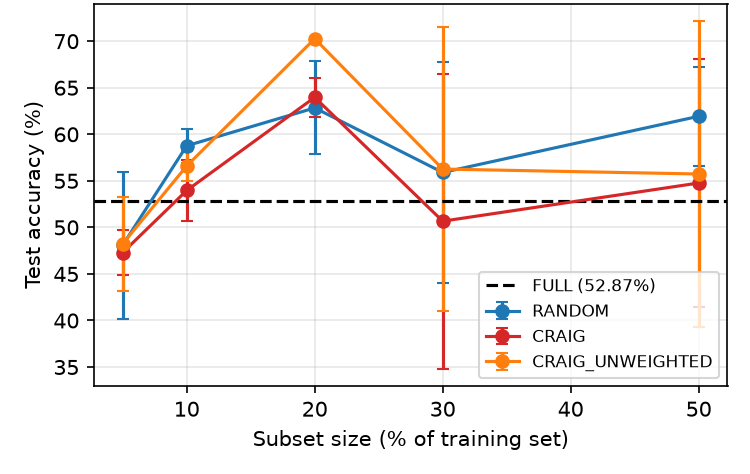
\includegraphics[width=\columnwidth]{ts_hard_acc_vs_ratio.png}
\caption{Synthetic time series, hard setting ($\sigma{=}2.0$): test accuracy vs.\ subset size (mean $\pm$ std, 3 seeds). The large error bars and the low FULL accuracy (52.87\%) show that this setting is not reliable for ranking methods.}
\label{fig:ts}
\end{figure}

\subsection{Scaling with dataset size}

Fig.~\ref{fig:scaling}a and the top of Table~\ref{tab:scaling} show that selection cost grows faster than full training. From $N{=}1{,}000$ to $20{,}000$ (a 20$\times$ increase), $\Tfull$ grows by 20.4$\times$, $\Tsel$ by 117.8$\times$, and the facility-location time by 368.4$\times$. From $10{,}000$ to $20{,}000$ alone, the facility-location time grows by 7.29$\times$, consistent with the quadratic size of the per-class similarity matrices and the cost of the greedy passes over them. The end-to-end speedup falls from 1.50$\times$ at $N{=}1{,}000$ to 1.12$\times$ at $5{,}000$, then to 0.75$\times$ at $10{,}000$ and 0.33$\times$ at $20{,}000$. \emph{The break-even point therefore lies between $N{=}5{,}000$ and $N{=}10{,}000$ in this setup.} At every size, CRAIG has the higher mean accuracy at the 10\% ratio (e.g., 76.66\% vs.\ 72.83\% at $N{=}1{,}000$ and 89.54\% vs.\ 89.05\% at $20{,}000$). The gap shrinks as $N$ grows. Only two seeds were run, so these gaps carry limited statistical weight.

\subsection{Scaling with sequence length}

The 1D CNN ends in global average pooling, so its parameter count, and hence the gradient dimension $D$, does not depend on $L$. As a result, the similarity and facility-location times stay roughly flat across $L$ (bottom of Table~\ref{tab:scaling}, Fig.~\ref{fig:scaling}b; the dip in similarity time at $L{=}1000$ was not investigated). Only the gradient computation grows: from 0.126\,s at $L{=}50$ to 1.499\,s at $L{=}1000$, an 11.9$\times$ increase. Full training also grows with $L$, from 1.058\,s to 5.328\,s, so CRAIG breaks even at every length (2.25--3.01$\times$). In accuracy, however, CRAIG is below RANDOM for $L\ge200$ (e.g., 54.60\% vs.\ 64.25\% at $L{=}1000$). The variances are large, and FULL itself drops to $84.35\pm10.39\%$ at $L{=}1000$.

%======================================================================
\section{Discussion}
\label{sec:discussion}
%======================================================================
\textbf{The weights matter.} The most robust result of this reproduction is the role of the Voronoi weights. On MNIST, the same CRAIG points used without weights give a larger gradient error than random sampling (Table~\ref{tab:mnist_gerr}) and lower accuracy at every ratio. On MNIST, weighted CRAIG beats unweighted CRAIG in every seed at every ratio (Table~\ref{tab:paired}). The medoids returned by facility location are, by construction, not a uniform sample. Treating them as one discards the information about how much of the data each medoid represents.

\textbf{Gradient matching is necessary but not sufficient.} On all three datasets, CRAIG achieves a lower gradient error than random sampling at the selection parameters. The improvement is modest on MNIST and large on CIFAR-10 and the time series. Accuracy follows only on MNIST, where the model is convex and the gradient geometry is stable during training. For the CNNs, a single selection at random initialization matches the gradients of an untrained network. This is a likely reason that the large gradient-error advantage on CIFAR-10 did not improve accuracy beyond the 10\% ratio.

\textbf{When does CRAIG pay off in time?} CRAIG pays off only when $\Tsel<\Tfull-\Tsub$. In our runs, this inequality is governed by three factors:
\begin{enumerate}
\item \emph{The greedy step dominates.} On MNIST, the pure-Python lazy greedy takes 77--81\% of $\Tsel$. Per-sample gradients via \texttt{vmap} cost only about 1\,s for 60k samples. Engineering effort should therefore target the greedy step, for example a compiled or vectorized implementation or a stochastic variant, rather than the gradient computation.
\item \emph{Per-class size matters more than total size.} Selection cost scales super-linearly in the per-class sample count, whereas full training scales linearly in $N$. In the dataset-size study, CRAIG is faster end-to-end up to $N{=}5{,}000$ and slower from $N{=}10{,}000$. On full MNIST (about 6,000 samples per class), selection alone takes 4.47--5.80$\times$ the full training time.
\item \emph{Cheap training makes break-even hard.} Full MNIST logistic regression trains in 6.58\,s on 8 CPU cores, which leaves very little time to save. The selection cost does not depend on the number of epochs, while $\Tfull-\Tsub$ grows with it, so longer training or more expensive models move the balance toward CRAIG. As a purely arithmetic illustration (not measured), the MNIST selection would have to be reused across about $\Tsel/(\Tfull-\Tsub)$ training runs of the same length to amortize: $29.41/6.12\approx4.8$ runs at 5\% and $38.20/2.43\approx15.7$ runs at 50\%. Such reuse is valid only if the subset stays useful across runs.
\end{enumerate}
In the CIFAR-10 and time-series settings, CRAIG does break even, because the gradient dimension or the per-class count is small. In those settings, however, uniform random subsets were at least as accurate and even cheaper, so the time saving alone is not an argument for CRAIG.

%======================================================================
\section{Limitations and Threats to Validity}
\label{sec:limitations}
%======================================================================
\begin{itemize}
\item \textbf{CPU-only, non-isolated hardware.} All runs used a shared 8-core CPU machine. Timing noise is visible: selection-time std is up to 7.17\,s on MNIST, and full-training-time std is 3.90\,s on CIFAR-10. GPU and MPS paths are untested. The relative cost of the stages, and therefore the break-even point, will differ on accelerators.
\item \textbf{Single, one-shot selection.} The subset is selected once from exact gradients at the initial weights. The original method re-selects during training for deep networks and uses feature-space bounds for convex models~\cite{mirzasoleiman2020craig}. Our deep-network results should therefore not be read as a test of the original per-epoch protocol.
\item \textbf{Simplified weighted training.} Our per-minibatch normalized weighted loss is a simplification of the weighted incremental-gradient updates in the original method.
\item \textbf{Reduced CIFAR-10.} We used 10k of the 50k training images, a small CNN, 10 epochs, no augmentation, and 3 seeds. FULL reaches only 59.02\%. These results are not comparable to published CIFAR-10 numbers.
\item \textbf{Synthetic time series.} We used no real time-series benchmark. The easy setting saturates at 100\%, and the hard setting is unstable, with FULL below several subsets. Neither supports conclusions about accuracy on real time-series data.
\item \textbf{Few seeds in places.} We used 3 seeds for CIFAR-10 and the time series and 2 for the scaling studies, which limits the statistical power of small accuracy differences. We report paired differences and win counts rather than significance tests.
\item \textbf{Unoptimized greedy.} The lazy greedy is written in Python with a binary heap. A faster implementation would shift the break-even point. We did not implement stochastic or distributed greedy variants.
\end{itemize}

%======================================================================
\section{Conclusion}
%======================================================================
We re-implemented CRAIG with exact vectorized per-sample gradients, blockwise similarity, lazy greedy facility location, and Voronoi weights, and evaluated it end-to-end on a CPU. On MNIST with logistic regression, the statistical claim reproduces: weighted CRAIG subsets have higher mean accuracy than random subsets of the same size at every ratio, and the weights are essential. The computational claim does not reproduce in our setting: selection costs 4.47--5.80$\times$ the full training time, giving an end-to-end speedup of only 0.16--0.22$\times$. The scaling study puts the break-even point between 5k and 10k training samples. With one-shot selection at initialization, CRAIG gave no reliable accuracy gain on reduced CIFAR-10 or on synthetic time series, despite much lower gradient approximation error. Natural next steps are a faster greedy implementation, per-epoch re-selection for deep networks, GPU timing, the full CIFAR-10 dataset, and real time-series benchmarks.

\bibliographystyle{IEEEtran}
\bibliography{references}

\end{document}
